\documentclass[11pt,helvetica,letter]{article}
%Opciones de idioma
\usepackage[spanish]{babel}
%Codificaci�n de los caracteres
\usepackage[utf8]{inputenc}
%S�mbolos matem�ticos
%Definiciones
\usepackage{amsmath, amssymb, amsthm}
\usepackage{wasysym}
\usepackage{graphicx}
\usepackage[dvipsnames,table,xcdraw]{xcolor}
%Tablas
\usepackage{tikz}
\usetikzlibrary{matrix}
% Defining some symbols:
\newcommand*\up{\textcolor{YellowGreen}{$\blacktriangle$}}
\newcommand*\down{\textcolor{Red}{$\blacktriangledown$}}
\newcommand*\const{\textcolor{darkgray}{\textbf{--}}}
\newcommand*\head[1]{\textbf{#1}}
% The table environment:
\newenvironment{matrixtable}[5]{%
  \begin{tikzpicture}[matrix of nodes/.style={
    execute at begin cell=\node\bgroup\strut,
    execute at end cell=\egroup;}]
  \matrix (m) [matrix of nodes,top color=gray!20,
    bottom color=gray!80,draw=white,
    nodes={draw,top color=white!10,bottom color=gray!35,
    draw=black,inner sep=0pt,minimum height=3.1ex},
    column sep=0.5ex,row sep=0.6ex,inner sep=2ex,
    column 1/.style={minimum width=#1},
    column 2/.style={minimum width=#2},
    column 3/.style={minimum width=#3},
    column 4/.style={minimum width=#4},
    column 5/.style={minimum width=#5}]}%
{;\end{tikzpicture}}

\newtheorem{theorem}{Teorema}
\newcommand{\ateq}[2]{
$\mathsf{at}(#1)=#2$
}
%Estilo de encabezados y pie de p�gina
\pagestyle{plain}
\title{Prueba low}
\author{
Tesista: David Gustavo Merinos Sosa \\
Directora de tesis: María Dolores Lara Cuevas
}
\date{}

%%%%%%%%%%%%%%%%%%%%%%%%%%%%%%%%%%%%%%
%%%%%%%%%%%%%%%%%%%%%%%%%%%%%%%%%%%%%%
%%%%%%%%%%%%%%%%%%%%%%%%%%%%%%%%%%%%%%

\begin{document}

\maketitle
\begin{theorem}
Para $n>4$, $\mathsf{at}(K_n)>2$.
\end{theorem}
\begin{proof}
  Supongamos \ateq{K_n}{2} con $n>4$. Esto implica que existen dos thrackles $T_1,T_2$
   tales que $|T_1 \cup T_2| \geq \binom{n}{2}$. En el mejor caso $T_1$ y $T_2$ son thrackles
   maximos y solo comparten una arista a pares. Entonces $|T_1 \cup T_2| \leq 2n-1$, luego para $n>4$
   tenemos que $\binom{n}{2}>6$.
   \begin{align*}
     2n-1 &\geq 6 \\
     2n &\geq 7 \\
     n &\geq 3.5 < 4 \enskip \text{\lightning}
   \end{align*}
   De esta contradicción decimos que para $K_n$ con $n>4$ su antithickness es mayor a 2.
\end{proof}

\section{Encontrar el anti-thickness geométrico de $K_n$}
Sea $K_n^i$ el dibujo de $K_n$ equivalente al tipo de orden $i$ para $n$ puntos. Supongamos que \ateq{K_n^i}{\lambda_i}.
Y que para este tipo de orden existen $M$ thrackles máximos. Sea $\Lambda_j$ con $j=1\dots\binom{M}{\lambda}$ una conjunto de
tamaño $\lambda$ de thrackles máximos. Definimos $m_i = |\bigcup \Lambda_j|$

Si sucede que $m_i > \binom{n}{2}$, podemos decir que el tipo de orden $i$ tiene
anti-thickness a lo sumo $\lambda$. El anti-thickness del tipo de orden $i$ es el $\lambda$ más pequeño
para el cual se cumple la condición anterior.

Si repetimos este análisis para cada dibujo de $K_n$, es decir, para cada tipo de orden, podemos decir que
el anti-thickness geométrico de $K_n$ es el $\lambda$ más pequeño resultante de todos los tipos de orden.

 % \begin{theorem}
 %   Para $n>6$, $\mathsf{at}(K_n)>3$.
 % \end{theorem}
 %
 % \begin{proof}
 %  Supongamos que \ateq{K_n}{2} con $n>6$. Esto implica que existen tres thrackles $T_1,T_2,T_3$
 %  tales que $|T_1 \cup T_2 \cup T_3| \geq \binom{n}{2}$. En el mejor caso $T_1,T_2$ y $T_3$ son máximos
 %  y comparten solo una arista a pares, decimos que $|T_1 \cup T_2 \cup T_3| \leq 3n - \binom{3}{2}$.
 %  Luego, para $n>6$ tenemos $\binom{n}{2} > 15$.
 %  \begin{align*}
 %    3n - 2 &\geq 15 \\
 %    3n &\geq 17  \\
 %    n &\geq 5.6 < 6 \enskip \text{\lightning}
 %  \end{align*}
 %\end{proof}
\section{Saber si $\mathsf{at}(K_n) > k$ para $n>6$}
Supongamos \ateq{K_n}{k} con $n>6$. Esto implica que existen $k$ thrackles $T_1,T_2,\dots T_k$
 tales que $|T_1 \cup T_2 \cup \dots T_k| \geq \binom{n}{2}$. En general, $|T_1 \cup T_2 \cup \dots T_k| \leq kn - m$
 donde $m$ es el total de aristas repetidas entre thrackles. Luego para $n>6$, $\binom{n}{2} > 15$
 tenemos que $\binom{n}{2}>6$. Esto nos da la siguiente desigualdad:
 \begin{align*}
   kn - m &\geq 15
 \end{align*}
 Lo que implica que \ateq{K_n}{k} cuando $m \leq kn-15$ para $n>6$.

 Por ejemplo, digamos que $k=3,n=7$ la anterior condición nos dice que el anti-thickness de $K_7$ será $3$ si $m \leq 6$. Basta con examinar cada pareja de thrackles cuya intersección es de tamaño 1, y compararla con cada uno de los otros thrackles de su complemento, contar las aristas repetidas y observar que en todos los casos se repiten mas de 6 aristas, es decir $m>6$. Por lo que podemos decir que $\mathsf{at^g}(K_7) > 3$. Y luego, como $\mathsf{cat}(K_7) = 4$, $\mathsf{at^g}(K_7) = 4$.

 \section{Estadísticas de repeticiones}
 \begin{center}
 \begin{matrixtable}{1.2cm}{1.2cm}{2.4cm}{1.5cm}{1.5cm}{
   \head{$n$}   & \head{OT} & \head{Dec. size} & \head{$min\_rep$} & \head{$max\_rep$}\\
   6 & 0    & 3 & 3 & 3 \\\hline\\
   7 & 0    & 4 & 7 & 7 \\\hline\\
   8 & 0      & 5 & 10 & 12\\
   8 & 12  & 5 & 12    & 12\\
   8 & 54    & 5  & 12  & 12\\\hline\\
   9 & 12  & 6  & 15    & 18\\
   9 & 52 & 6  & 17    & 17\\
   9 & 54     & 6  & 16    & 18\\
   9 & 80   & 6  & 14    & 14\\
   9 & 696      & 6  & 18  & 18\\
   9 & 1080      & 6  & 16  & 16\\
   9 & 1287      & 6  & 15  & 17\\}
 \end{matrixtable}
 \end{center}\leavevmode\\
 \section{ Lema }
 \begin{theorem}
   Dados dos thrackles máximos $T_1$ y $T_2$, su intersección en aristas es no vacía.
 \end{theorem}
 \begin{proof}
 Sea $T_1$ un thrackle máximo con $C_1=V(C(T_1))$, seleccionamos $k$ vértices tales que no estén en $C_1$ y con $k$ impar
 para formar un ciclo impar $C_2$, cuyas cuñas contengan a $P-\{C_2\}= C_1$ y que además $C_1 \cap C_2 = \emptyset$. Necesariamente
 todo $v \in C_2$ es un vértice de grado 1 de $T_1$.

 Entonces existen aristas de $T_1$ tales que inciden en vértices de $C_2$, o lo que es igual,
 aristas salientes de $C_1$ que acaban en $C_2$. Como las cuñas generadas por vértices de $C_2$ contienen a todo $C_1$ y las
 cuñas generadas por vértices de $C_1$ contienen a todo $C_2$, entonces existe una arista $e\in T_1$
 tal que $e\in W_{T_1}(u) \cap W_{T_2}(v)$ con $u\in C_1, v\in C_2$. Notese que esta arista equivalentemente sale de algún vértice
 $v \in C_2$ y acaba en algún vértice $u \in C_2$.

 Finalmente si decimos que $T_2 = C_2$ y luego agregamos todas las aristas que salgan de cuñas generadas por vértices de $C_2$
 y acaban en vértices de $C_1$, lo cual es posible por construcción, tenemos que \[T_2 \ni  e, \Rightarrow T_2 \cap T_1 \ni e \Rightarrow T_2 \cap T_1 \neq \emptyset\]
\end{proof}

\begin{figure}[h]
  \centering
  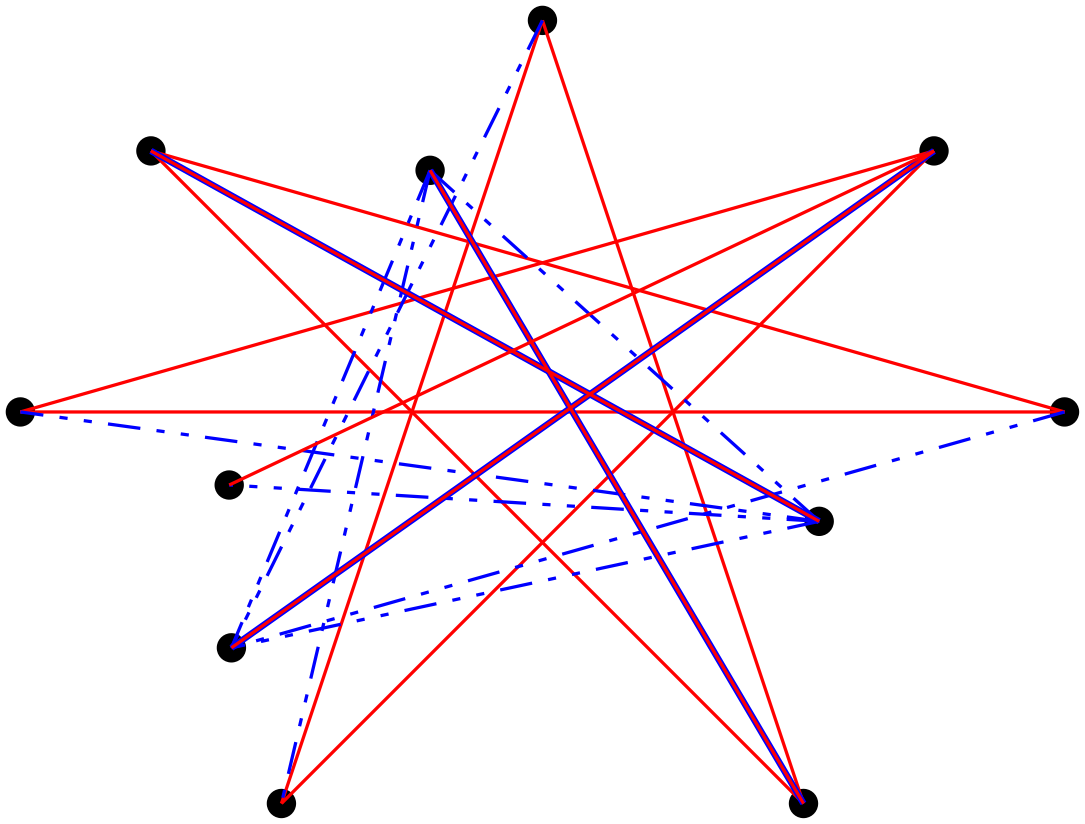
\includegraphics[width=8cm]{lemathrackles}

\end{figure}
\newpage
\section{Doble contención}
Caso en el que $C_2$ está contenido en la unión de exactamente 2 cuñas de $C_1$.\\
Sean $u,u'$ vértices de $C_1$ cuyos ápices cubren a todo $C_2$:
\[ \exists! v\in C_2: v \text{ ve a } u \]
\[ \exists! v'\in C_2: v' \text{ ve a } u' \]
Si $v=v'$ entonces $v$ ve a $u$ y $v$ ve a $u'$, luego $u$ ve a $v$ o $u'$ ve a $v$ y hay doble contención.\\
Si $v\neq v$ entonces $u$ ve a $v'$ y $u'$ ve a $v$, obviando la doble contención tenemos que suponer además que
$u$ no ve a $v$ y $u'$ no ve a $v'$.

\begin{figure}[h]
  \centering
  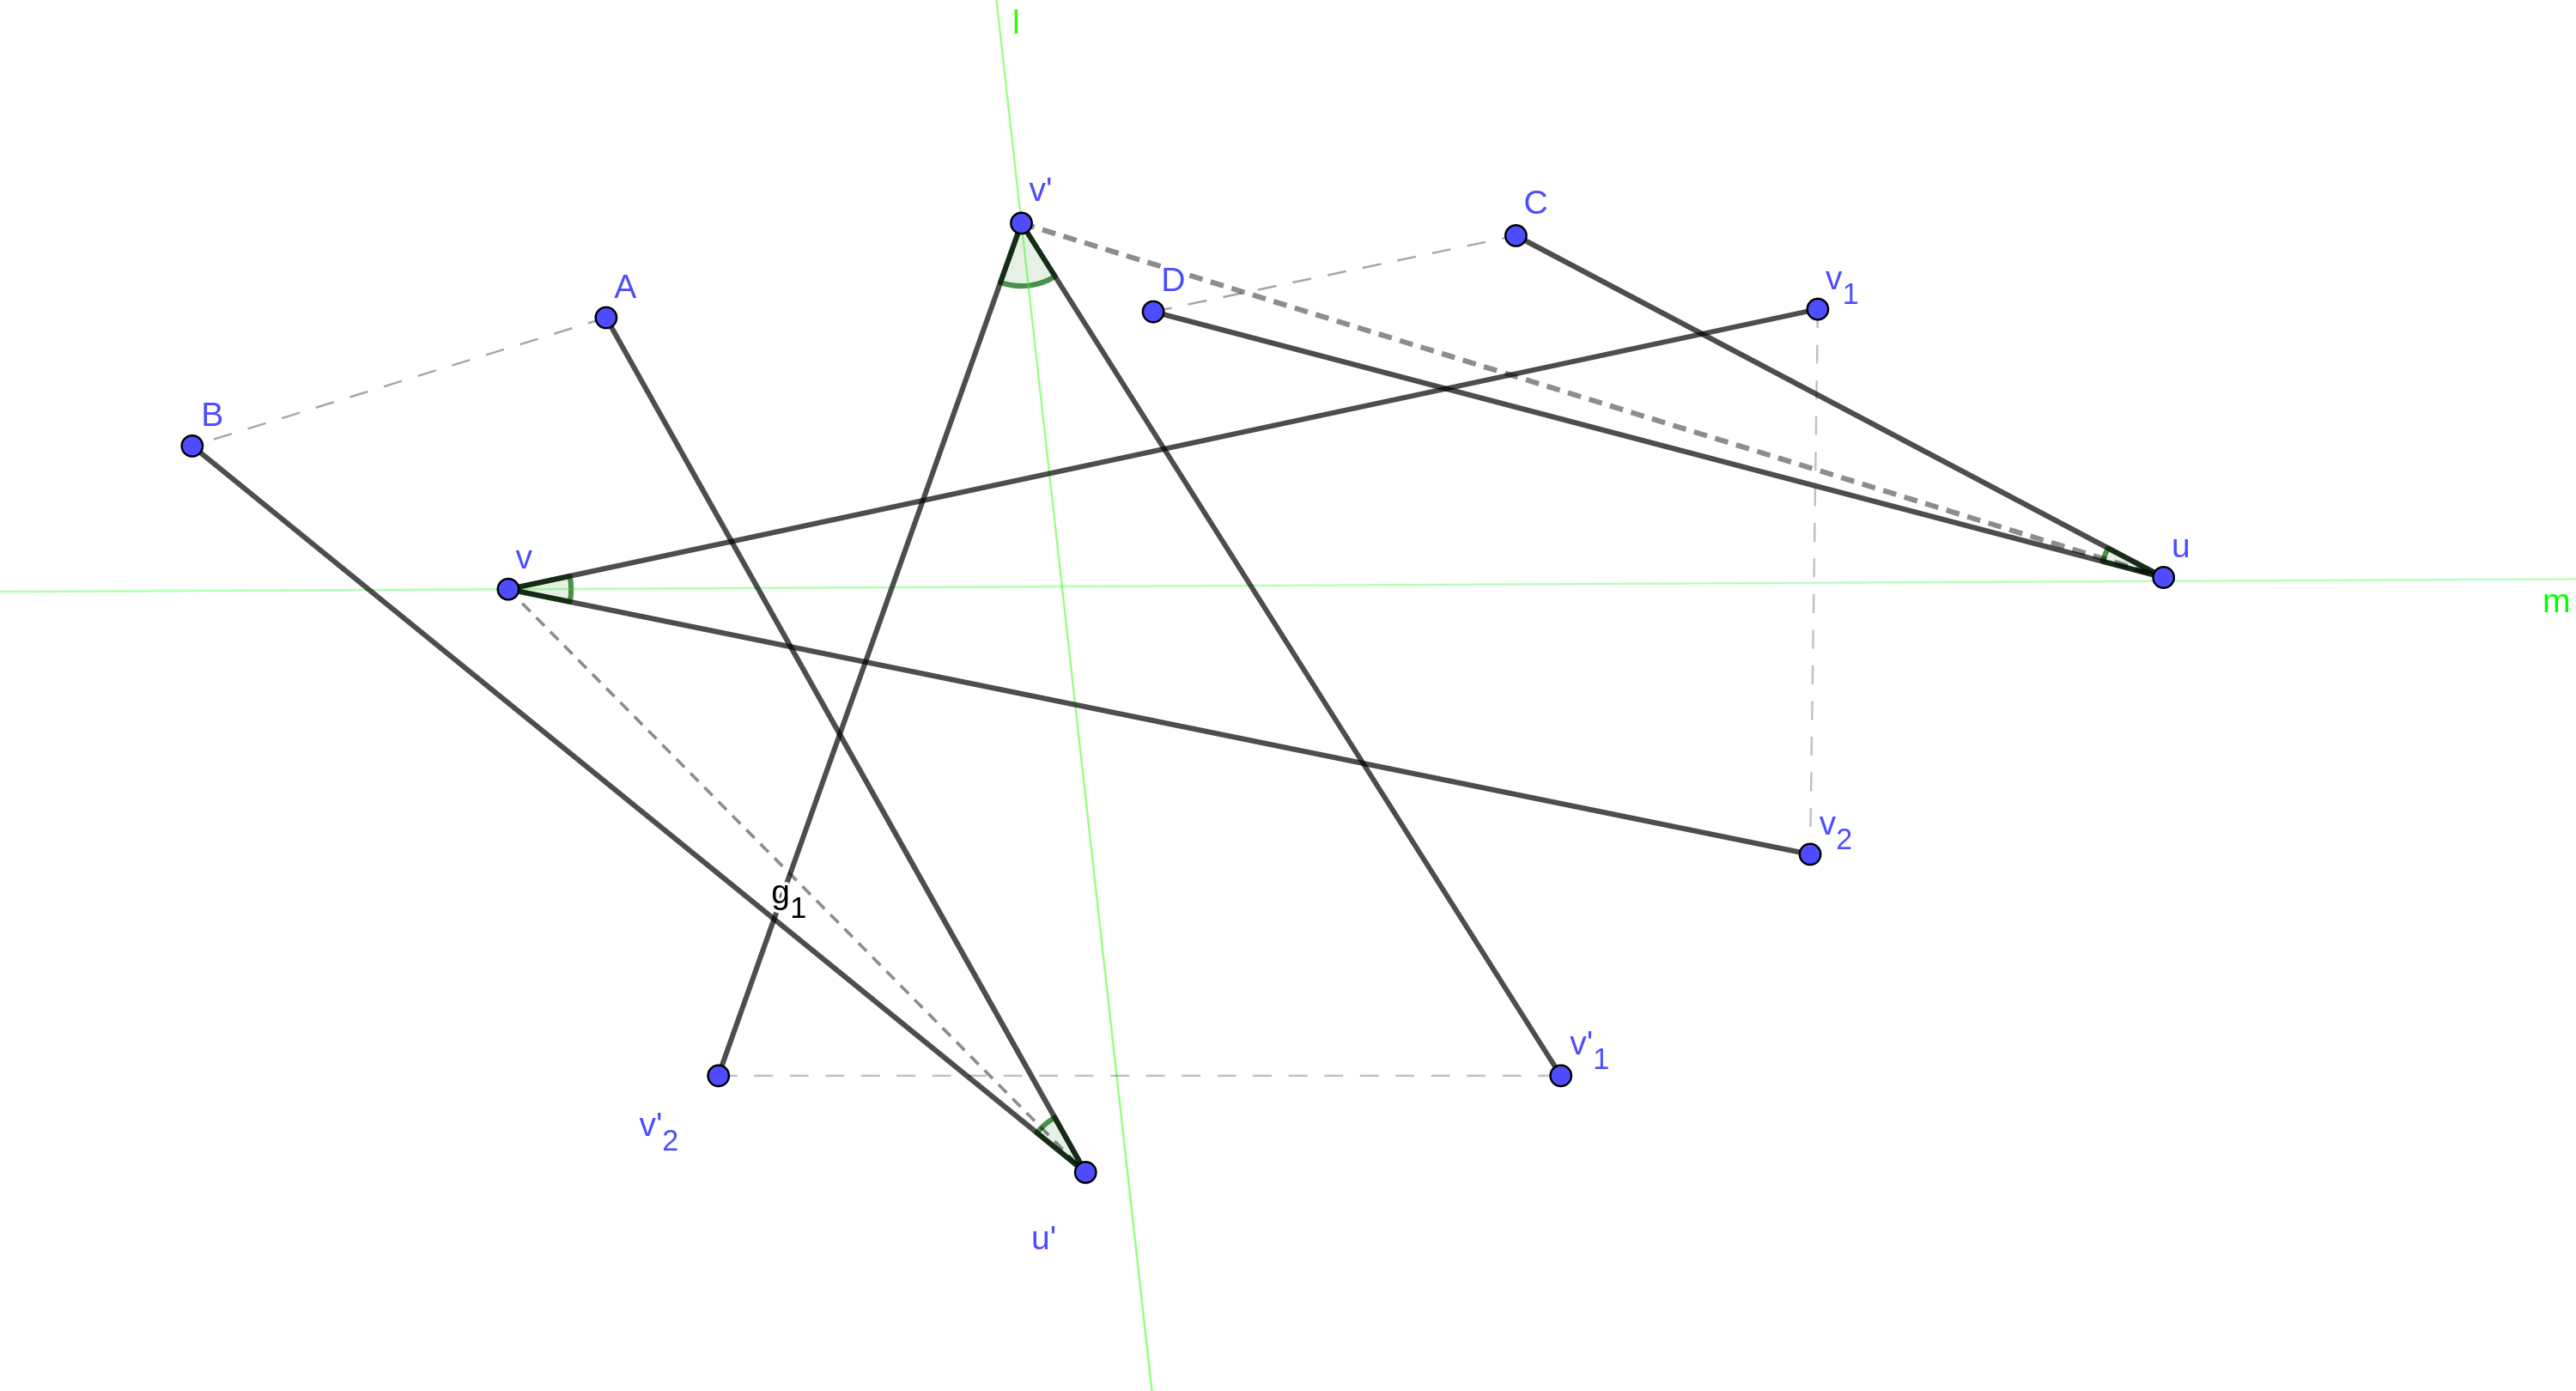
\includegraphics[width=12cm]{doble_contencion}
\end{figure}
\end{document}
